\subsection{Logistic Regression}

We have applied logistic regression to our data. For logistic regression, we calculate a value for each data object. This value can be used to estimate the likelihood of the object to be CHD positive.

\begin{figure}
	\begin{subfigure}[b]{0.5\textwidth}
	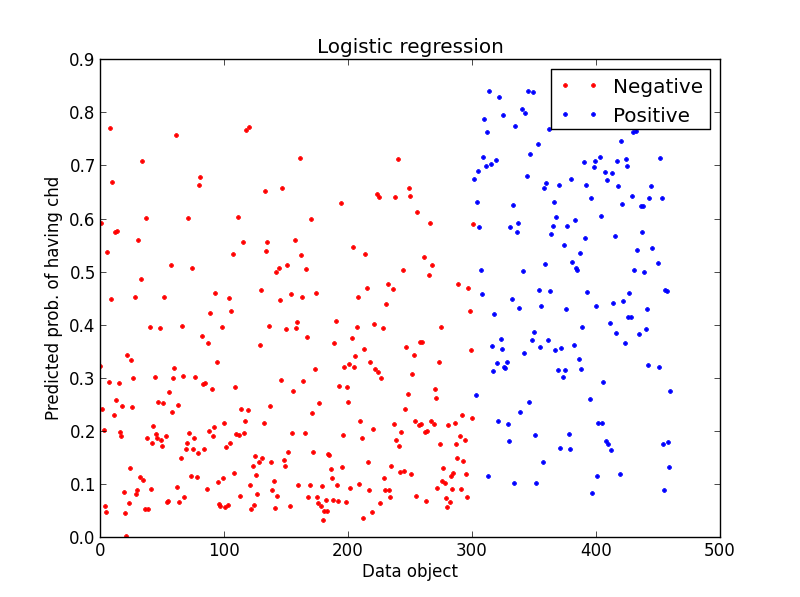
\includegraphics[scale=0.4]{pictures/logisticregressionX.png}
	\caption{Looking at all attributes.}
	\label{logicalRegressionResultX}
	\end{subfigure}
	\begin{subfigure}[b]{0.5\textwidth}
	\includegraphics[scale=0.4]{pictures/logisticregressionXad.png}	
	\caption{Looking at attributes selected by forward selection.}
	\label{logicalRegressionResultXad}
	\end{subfigure}

	\begin{subfigure}[b]{0.5\textwidth}
	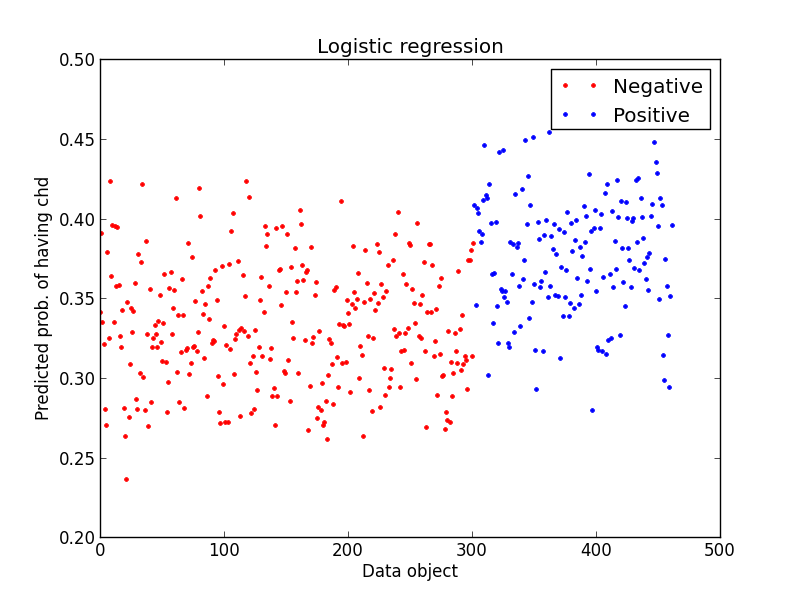
\includegraphics[scale=0.4]{pictures/logisticregressionXPC.png}
	\caption{Looking at all principal components.}
	\label{logicalRegressionResultXPA}
	\end{subfigure}
	\begin{subfigure}[b]{0.5\textwidth}
	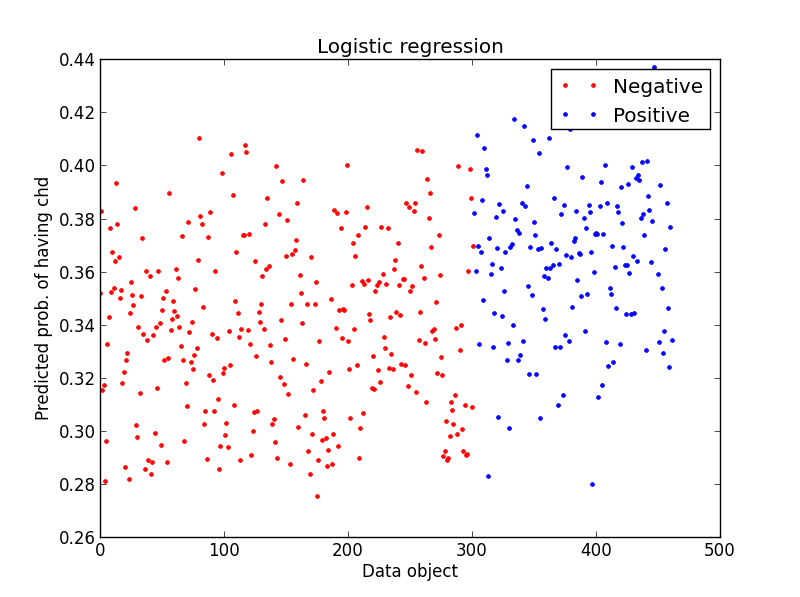
\includegraphics[scale=0.4]{pictures/logisticregressionX2PC.png}
	\caption{Looking at two most important principal components.}
	\label{logicalRegressionResultX2PA}
	\end{subfigure}
\caption{This figure shows results of performing logical regression for different input.}
\label{logicalRegressionResults}
\end{figure}

Se Figure \ref{logicalRegressionResults} to see output for our different input, when running Logistic Regression. Looking at Figure \ref{logicalRegressionResultX}, we see our results, when we have not alternated with the data, and likewise we see at Figure \ref{logicalRegressionResultXad}, our results for when, we have removed the attributes with less influence, meaning for this case we only look at the attributes: Age, Alcohol, Type-A, Family history, Low density lipoprotein cholesterol (LDL). For see especially from these to output of results that there is a tendency for subjects actually having the disease to have a higher probability of having the disease, even though we still see subjects having the disease with low predicted probability and likewise subjects not having the disease having a high predicted probability.

Looking at Figures \ref{logicalRegressionResultXPA} and \ref{logicalRegressionResultX2PA}, where we use principal components to give a logical regression of the data, also see a tendency of people actually having the disease, also have a higher predicted probability of having the disease. However we see that the interval of predicted probabilities are much less. Actually we see from these two graphs that all subjects have a predicted probability of less than 50\%.

A naive way of classifying subjects from these results, is classifying subjects with a predicted probability of more than 50\% as CHD-positive and vice versa the rest as being CHD-negative. This way we can go through all the subjects of the sets, and see how big a percentage are classified correct or wrong. This gives us the misclassification rate. These can be seen in Figure

\begin{table}
\begin{longtable}{lc} \hline
Figure \ref{logicalRegressionResultX} & 26,6\% \\ 
Figure \ref{logicalRegressionResultXad} & 25,8\% \\ 
Figure \ref{logicalRegressionResultXPA} & 34,6\% \\ 
Figure \ref{logicalRegressionResultX2PA} & 34,6\% \\ \hline
\end{longtable}
\end{table}

We see that we actually get the smallest misclassification rate, when we look at the results from when we do not use principal component analysis, but we also see that in this case, we can use the results from our forward selection to decrease the misclassification result. For comparing these misclassification rates, we should compare to just classifying all objects to be negative. For this we get a misclassification rate of $\frac{160}{462}=34,6\%$, as we have 160 positive samples from a total of 462 samples. We see that this misclassification rate corresponds to the results described in Figures \ref{logicalRegressionResultXPA} and \ref{logicalRegressionResultX2PA}. This makes sense, since the predicted probability of all subjects in these cases are below 50\%.